\documentclass[]{report}

\usepackage{pdfpages} 
\usepackage[utf8]{inputenc}
\usepackage[spanish]{babel}

% Title Page
\title{Tema de tesis}
\author{Estudiante}


\begin{document}
	
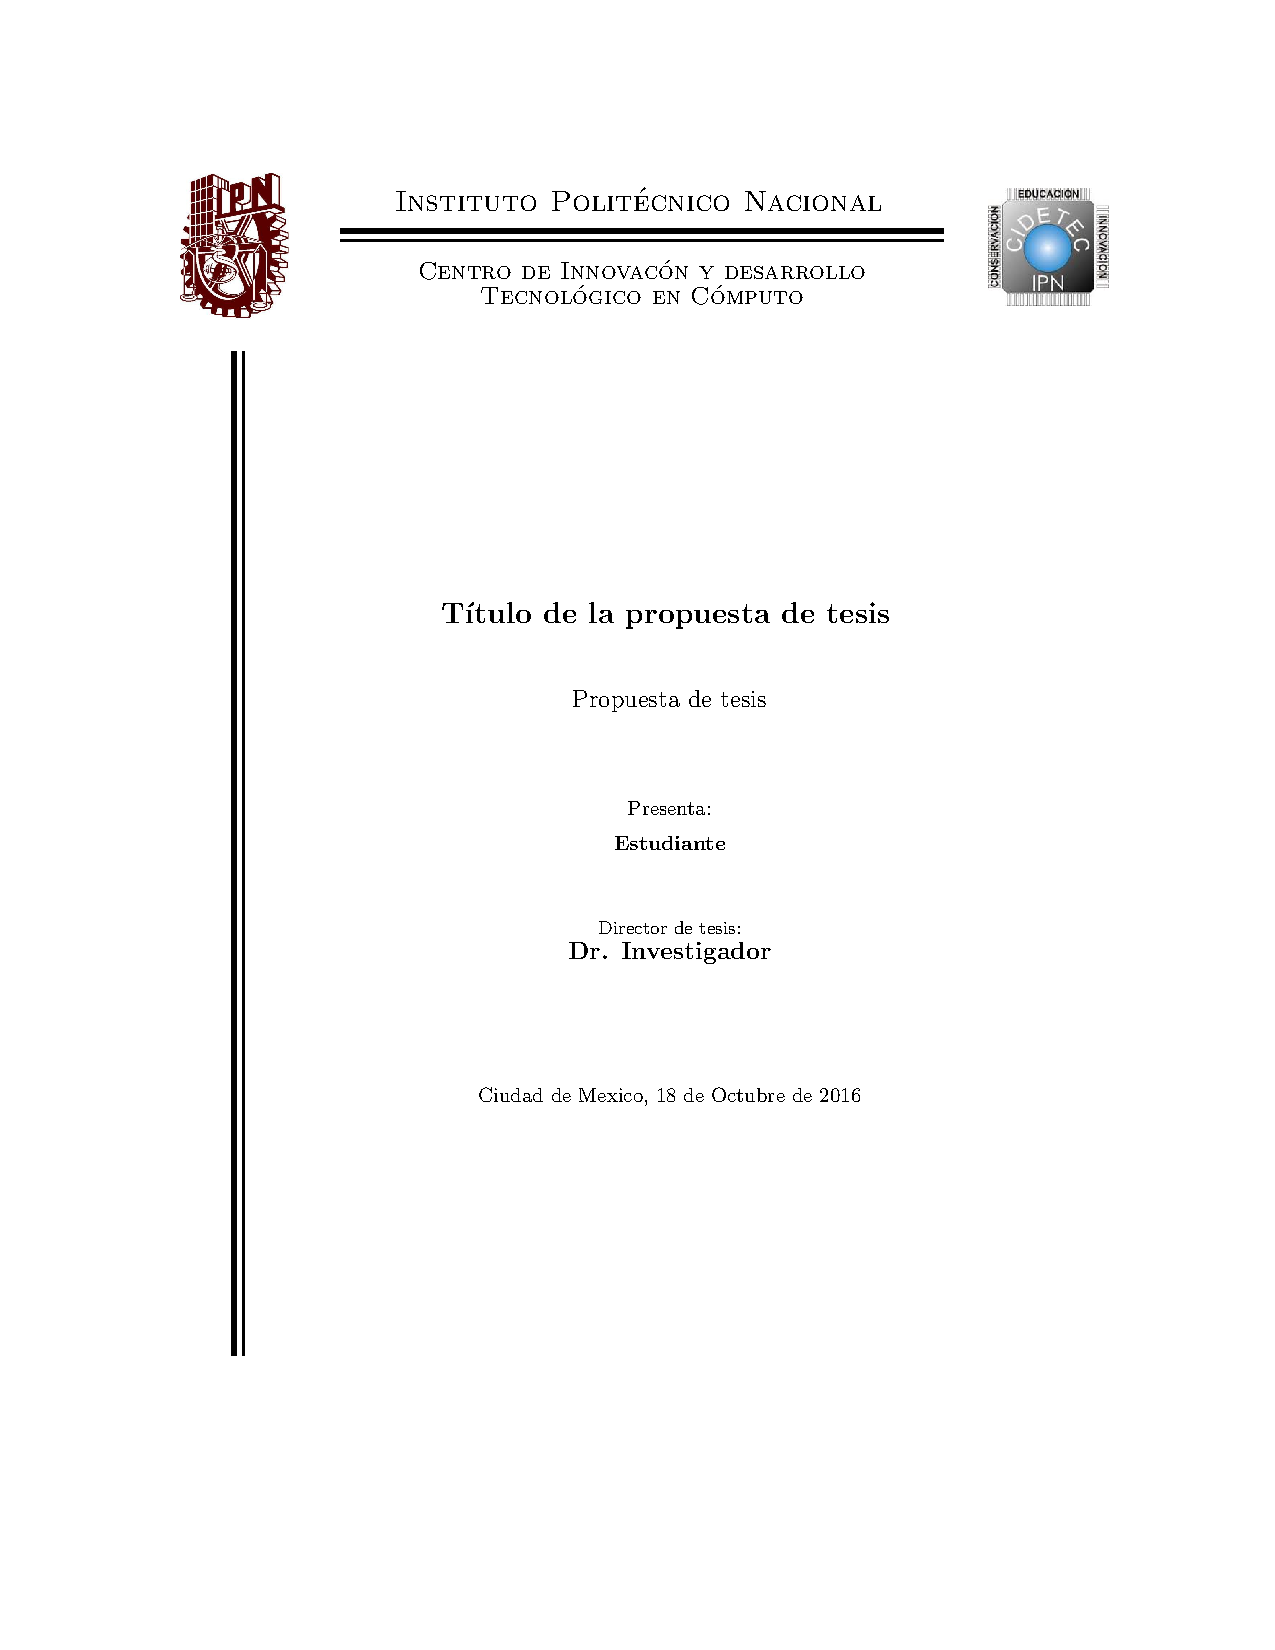
\includepdf[pages={1}]{portada.pdf}
	

\newpage\null\thispagestyle{empty}\newpage
	
%\maketitle

\begin{abstract}
	Aqui va el resumen 
\end{abstract}

\newpage\null\thispagestyle{empty}\newpage

\addtocontents{toc}{\hfill \textbf{Página} \par}
\tableofcontents

\chapter{Introducción}
\section{Motivación}
\section{Problema}

\chapter{Trabajo Relacionado}

\chapter{Propuesta}

\section{Hipótesis}
\section{Objetivo General}
\section{Metodología}
\subsection{Cronograma}

\chapter{Avances}

\chapter{Conclusiones}

\end{document}          
